\begin{frame}
    \frametitle{Objectifs : Le projet eSWARM}
    \begin{columns}[c]
        \begin{column}{0.6\textwidth}
            \begin{itemize}
                \item Stage dans la continuité du projet \textbf{eSWARM}.
                \item \textbf{Objectif global :} développer un système de drones quadricoptères \textbf{modulaire} et \textbf{reconfigurable}.
                \item Capable de s'assembler en vol pour des missions complexes (ex: transport de charges lourdes).
                \item \textbf{Inspiration :} projet ModQuad \cite{saldana_modquad_2018}, un essaim de drones reconfigurable.
            \end{itemize}
        \end{column}
        \begin{column}{0.4\textwidth}
            \begin{figure}
                \centering
                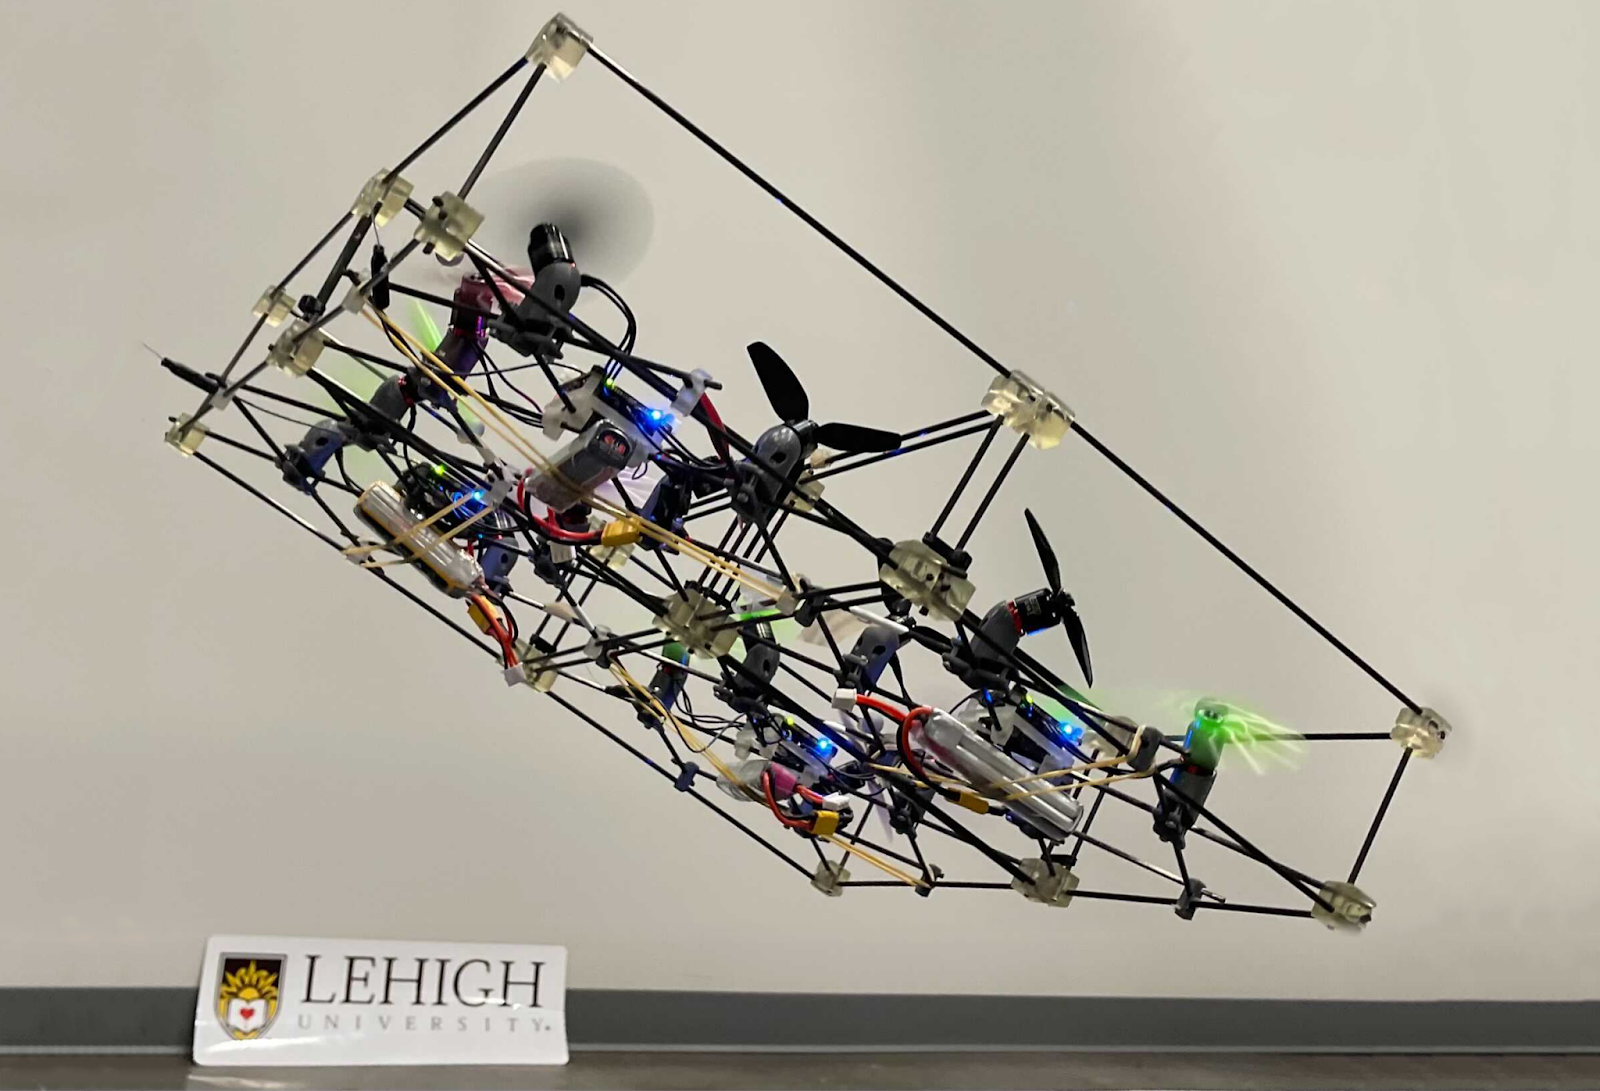
\includegraphics[width=\linewidth]{2-Introduction/pic/modquad.png}
                \caption{Système ModQuad \cite{saldana_modquad_2018}.}
            \end{figure}
        \end{column}
    \end{columns}
\end{frame}


\begin{frame}
    \frametitle{Objectifs : Cadre du stage}
    \begin{columns}[c]
        \begin{column}{0.6\textwidth}
            \begin{itemize}
                \item \textbf{Simplification :} Remplacement des drones par des robots terrestres holonomes.
                \item \textbf{Objectifs du stage :}
                \begin{enumerate}
                    \item Développer la plateforme de robots terrestres.
                    \item Mettre en place une architecture logicielle distribuée (ROS2).
                    \item Optimiser la commande distribuée de l'essaim.
                \end{enumerate}
            \end{itemize}
        \end{column}
        \begin{column}{0.4\textwidth}
            \begin{figure}
                \centering
                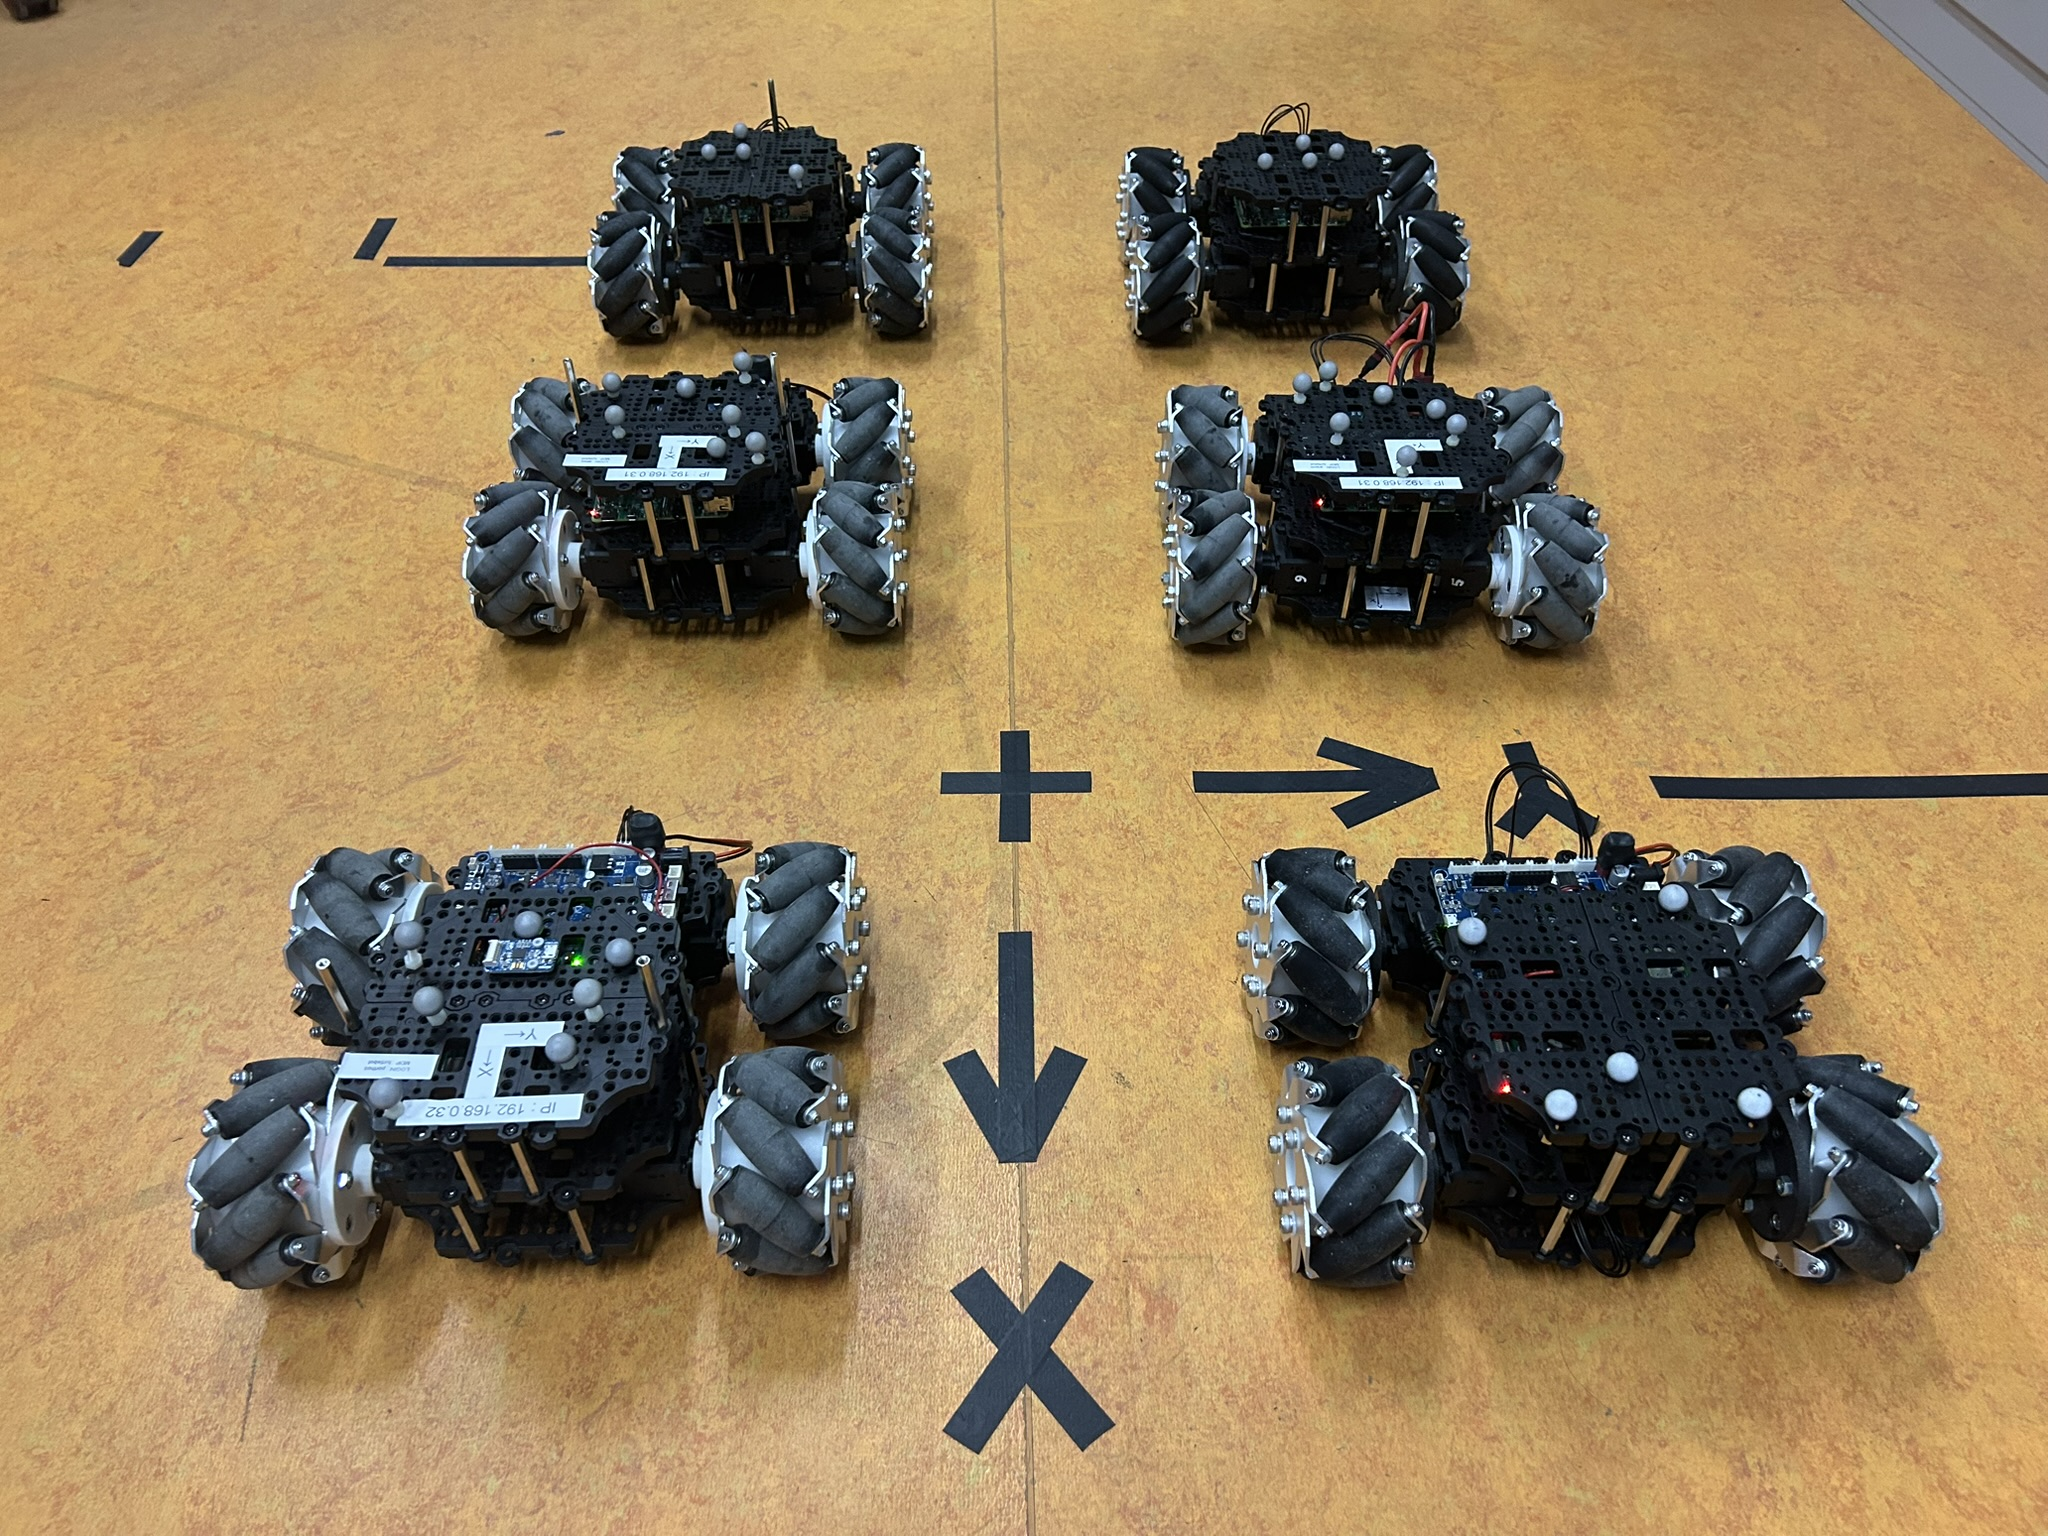
\includegraphics[width=\linewidth]{2-Introduction/pic/essaim.JPEG}
                \caption{Plateforme expérimentale de robots terrestres.}
            \end{figure}
        \end{column}
    \end{columns}
\end{frame}

\begin{frame}
    \frametitle{Objectifs : Aspect recherche}
    \begin{itemize}
        \item \textbf{Aspect recherche :}
        \begin{itemize}
            \item Comment optimiser la consommation énergétique des robots ?
            \item Comment minimiser les échanges d'informations entre les modules ?
        \end{itemize}
        \item \textbf{Approche proposée :}
        \begin{itemize}
            \item Implémentation de paradigmes de \textbf{commande événementielle} (Event-Triggered Control).
            \item Analyse des performances des algorithmes testés.
        \end{itemize}
    \end{itemize}
\end{frame}
